%%gji_extra_guide.tex
% \documentclass[extra,mreferee]{gji}
% \usepackage{mathrsfs,amsmath}
% \usepackage{timet}

\documentclass[a4paper, 11pt]{article}
\usepackage[pdftex]{graphicx}
\usepackage{fullpage}
\usepackage{mathrsfs,amsmath}
\usepackage{framed, color, fancybox}

\author{Seogi Kang and Douglas W. Oldenburg}  
\title{On recovering distributed IP information in airborne time domain electromagnetic data} 


%% =============================================================================
%% My equations
%% =============================================================================

\renewcommand{\div}{\nabla\cdot}
\newcommand{\grad}{\vec \nabla}
\newcommand{\curl}{{\vec \nabla}\times}
\newcommand {\J}{{\vec J}}
\renewcommand{\H}{{\vec H}}
\newcommand {\E}{{\vec E}}
\newcommand{\siginf}{\sigma_\infty}
\newcommand{\dsig}{\triangle\sigma}
\newcommand{\dcurl}{{\mathbf C}}
\newcommand{\dgrad}{{\mathbf G}}
\newcommand{\Acf}{{\mathbf A_c^f}}
\newcommand{\Ace}{{\mathbf A_c^e}}
\renewcommand{\S}{{\mathbf \Sigma}}
\newcommand{\St}{{\mathbf \Sigma_\tau}}
\newcommand{\T}{{\mathbf T}}
\newcommand{\Tt}{{\mathbf T_\tau}}
\newcommand{\diag}{\mathbf{diag}}
\newcommand{\M}{{\mathbf M}}
\newcommand{\MfMui}{{\M^f_{\mu^{-1}}}}
\newcommand{\MfMuoi}{{\M^f_{\mu_0^{-1}}}}
\newcommand{\dMfMuI}{{d_m (\M^f_{\mu^{-1}})^{-1}}}
\newcommand{\dMfMuoI}{{d_m (\M^f_{\mu_0^{-1}})^{-1}}}
\newcommand{\MeSig}{{\M^e_\sigma}}
\newcommand{\MeSigInf}{{\M^e_{\sigma_\infty}}}
\newcommand{\MeSigInfEtab}{{\M^e_{\sigma_\infty \bar{\eta}}}}
\newcommand{\MeSigInfEtat}{{\M^e_{\sigma_\infty \peta}}}
\newcommand{\MedSig}{{\M^e_{\triangle\sigma}}}
\newcommand{\MeSigO}{{\M^e_{\sigma_0}}}
\newcommand{\Me}{{\M^e}}
\newcommand{\Js}{\mathbf{J}^s}
\newcommand{\Mes}[1]{{\M^e_{#1}}}
\newcommand{\Mee}{{\M^e_e}}
\newcommand{\Mej}{{\M^e_j}}
\newcommand{\BigO}[1]{\mathcal{O}\bigl(#1\bigr)}
\newcommand{\bE}{\mathbf{E}}
\newcommand{\bEp}{\mathbf{E}^p}
\newcommand{\bB}{\mathbf{B}}
\newcommand{\bBp}{\mathbf{B}^p}
\newcommand{\bEs}{\mathbf{E}^s}
\newcommand{\bBs}{\mathbf{B}^s}
\newcommand{\bH}{\mathbf{H}}
\newcommand{\B}{\vec{B}}
\newcommand{\D}{\vec{D}}
\renewcommand{\H}{\vec{H}}
\newcommand{\s}{\vec{s}}
\newcommand{\bfJ}{\bf{J}}
\newcommand{\vecm}{\vec m}
\renewcommand{\Re}{\mathsf{Re}}
\renewcommand{\Im}{\mathsf{Im}}
\renewcommand {\j}  { {\vec j} }
\newcommand {\h}  { {\vec h} }
\renewcommand {\b}  { {\vec b} }
\newcommand {\e}  { {\vec e} }
\renewcommand {\d}  { {\vec d} }
\renewcommand {\u}  { {\vec u} }

\renewcommand {\dj}  { {\mathbf{j} } }
\renewcommand {\dh}  { {\mathbf{h} } }
\newcommand {\db}  { {\mathbf{b} } }
\newcommand {\de}  { {\mathbf{e} } }

\newcommand{\vol}{\mathbf{v}}
\newcommand{\I}{\vec{I}}
\newcommand{\A}{\mathbf{A}}
\newcommand{\bI}{\mathbf{I}}
\newcommand{\bus}{\mathbf{u}^s}
\newcommand{\brhss}{\mathbf{rhs}_s}
\newcommand{\bup}{\mathbf{u}^p}
\newcommand{\brhs}{\mathbf{rhs}}
%%-------------------------------
\newcommand{\bon}{b^{on}(t)}
\newcommand{\bp}{b^{p}}
\newcommand{\dbondt}{\frac{db^{on}(t)}{dt}}
\newcommand{\dfdt}{\frac{df(t)}{dt}}
\newcommand{\dfdtdsiginf}{\frac{\partial\frac{df(t)}{dt}}{\partial\siginf}}
\newcommand{\dfdsiginf}{\frac{\partial f(t)}{\partial\siginf}}
\newcommand{\dbgdsiginf}{\frac{\partial b^{Impulse}(t)}{\partial\siginf}}
\newcommand{\digint}{\frac{2}{\pi}\int_0^{\infty}}
\newcommand{\Gbiot}{\mathbf{G}_{Biot}}
%%-------------------------------
\newcommand{\peta}{\tilde{\eta}}
\newcommand{\eFmax}{\e^{\ F}_{max}}
\newcommand{\eref}{\e^{\ ref}}
\newcommand{\jref}{\j^{\ ref}}
\newcommand{\dip}{d^{IP}}
\newcommand{\sigpert}{\delta\sigma}

%% =============================================================================
%% End of my equations
%% =============================================================================


% \title[] {On recovering distributed IP information in airborne time domain electromagnetic data} 
% \author[] {Seogi Kang and Douglas W. Oldenburg}  
% \newcommand{\btx}{\textsc{BibTeX}}

\begin{document}
\maketitle
\tableofcontents
\clearpage

\section{Introduction}

The electrical conductivity of earth materials can be frequency dependent with the effective conductivity decreasing with decreasing frequency due to the buildup of electric charges that occur under the application of an electric field.
Effectively, the rock is electrically polarized. Finding this induced polarization (IP) response has been important in mineral exploration but it is also important in environmental problems, groundwater flow, and site characterization. 
Polarization charges can accumulate whenever there is an electric field in a medium and so the transmitter can be a galvanic or inductive source. 
Different excitation mechanisms originated from these two different sources, makes a principal difference in IP effects. 
Since the inductive source is divergence-free it does not have any steady-state electric field, whereas galvanic source has one. 
Understanding of IP effects for the galvanic source has been well-established for several decades (\cite{seigel1959}, \cite{seigel1974}). Especially for the restoration of the chargeability, linearized kernel function has been used assuming no EM induction effects (\cite{doug1994}). For the inductive source IP (ISIP), similar linearized approach to recover 3D IP information has been investigated for the frequency domain data (\cite{Marchant2012b}). However, recovering 3D IP information from the time domain EM (TEM) data, has not been carefully studied. 
Our focus in this article is upon the potential for extracting IP information from airborne TEM (ATEM) systems such as the coincident loop instrument. The observed data for this system often have negative transients (Mt Milligan, TKC). \cite{Weidelt1982} showed that the most plausible explanation of these is that they are caused by IP effects. 

To extract distributed IP information from the ATEM data, we use similar linearized inversion approach (Seigel , Doug), which has extensively been used in the industry. Application of this to the ATEM case will include three principal steps: 1) Restoration of the 3D conductivity, 2) EM decoupling, and 3) 3D IP inversion with linearized kernel function. 
The first step is not trivial because the observed ATEM data can be contaminated by IP effect . 
Similarly, the second step which requires conductivity is also challenging. Although these steps are essential elements of the 3D IP inversion of ATEM data and should be carefully investigated, we focus on the third step in this paper. 
Evaluating the linearization of IP responses for the ATEM case, and its validation are essential factors to perform the 3D IP inversion. 
In addition, the difference of the IP response on the inductive source from the galvanic source should be carefully incorporated to the linearized kernel.  

To demonstrate a 3D IP inversion procedure to recover distributed IP information from the ATEM data, in this article, we first define IP datum by decomposing the observed EM response. 
Based on this, then we develop a linearized kernel of IP responses for the ATEM data. 
Next, we suggest a 3D IP inversion methodology to recover multiple time channels of the pseudo-chargeability, and also investigate a potential to extract intrinsic Cole-Cole parameters from pseusdo-chargeability. Finally, we carefully analyze and validate each step of our 3D IP inversion procedure with numerical examples. 
      
    
%% =============================================================================
%% Section. Complex conductivity
%% =============================================================================

\subsection{Complex conductivity}
An often-used representation for complex conductivity in the frequency domain is the Cole-Cole model \cite{COLE}:
\begin{equation}
  \sigma(\omega) = \sigma_{\infty} - \sigma_{\infty}\frac{\eta}{1+(1-\eta)(\imath\omega\tau)^c} = \sigma_{\infty} + \triangle\sigma(\omega),
  \label{eq: sigma_freq}
\end{equation}
where $\sigma_{\infty}$ is the conductivity at infinite frequency, $\eta$ is the intrinsic chareability, $\tau$ is the time constant and $c$ is the frequency dependency. Real and imaginary parts of complex conductivity in frequency domain are shown in Figure ~\ref{Fig:FDandTDCole}(a) with Cole-Cole parameters: $\siginf$ = $10^{-2}$ S/m, $\eta $ = 0.5, $\tau$ = 0.01 and $c$=1. By applying inverse Fourier transform with time dependency, $e^{\imath\omega t}$, we have
\begin{equation}
  \sigma(t) = \mathscr{F}^{-1}[\sigma(\omega)] = \sigma_{\infty}\delta(t) + \triangle\sigma(t)
  \label{eq: sigma_time}
\end{equation}
where $\delta(t)$ is Dirac delta function and $\mathscr{F}^{-1}[\cdot]$ is inverse Fourier transform operator. Computation of $\triangle\sigma(t)$ can be convenient by assuming $c=1$, which is usually called Debye model. By evaluating inverse Fourier transform of $\triangle\sigma(\omega)$ when $c=1$, we have
\begin{equation}
  \sigma(t) = \sigma_{\infty}\delta(t) - \siginf\peta^{I}(t),
  \label{eq: sigma_time_c1}
\end{equation}
where intrinsic pseudo-chargeability, $\peta^{I}(t)$ is
\begin{equation}
    \peta^{I}(t) = -\frac{\dsig(t)}{\siginf}. %=\frac{\eta}{(1-\eta)\tau}e^{-\frac{t}{(1-\eta)\tau}}u(t)
    \label{eq: intrinsic_peta}
\end{equation}
Cole-Cole model in time domain is also shown in Figure ~\ref{Fig:FDandTDCole}. Used Cole-Cole parameters here are same as the above.

\begin{figure}
  \centering
  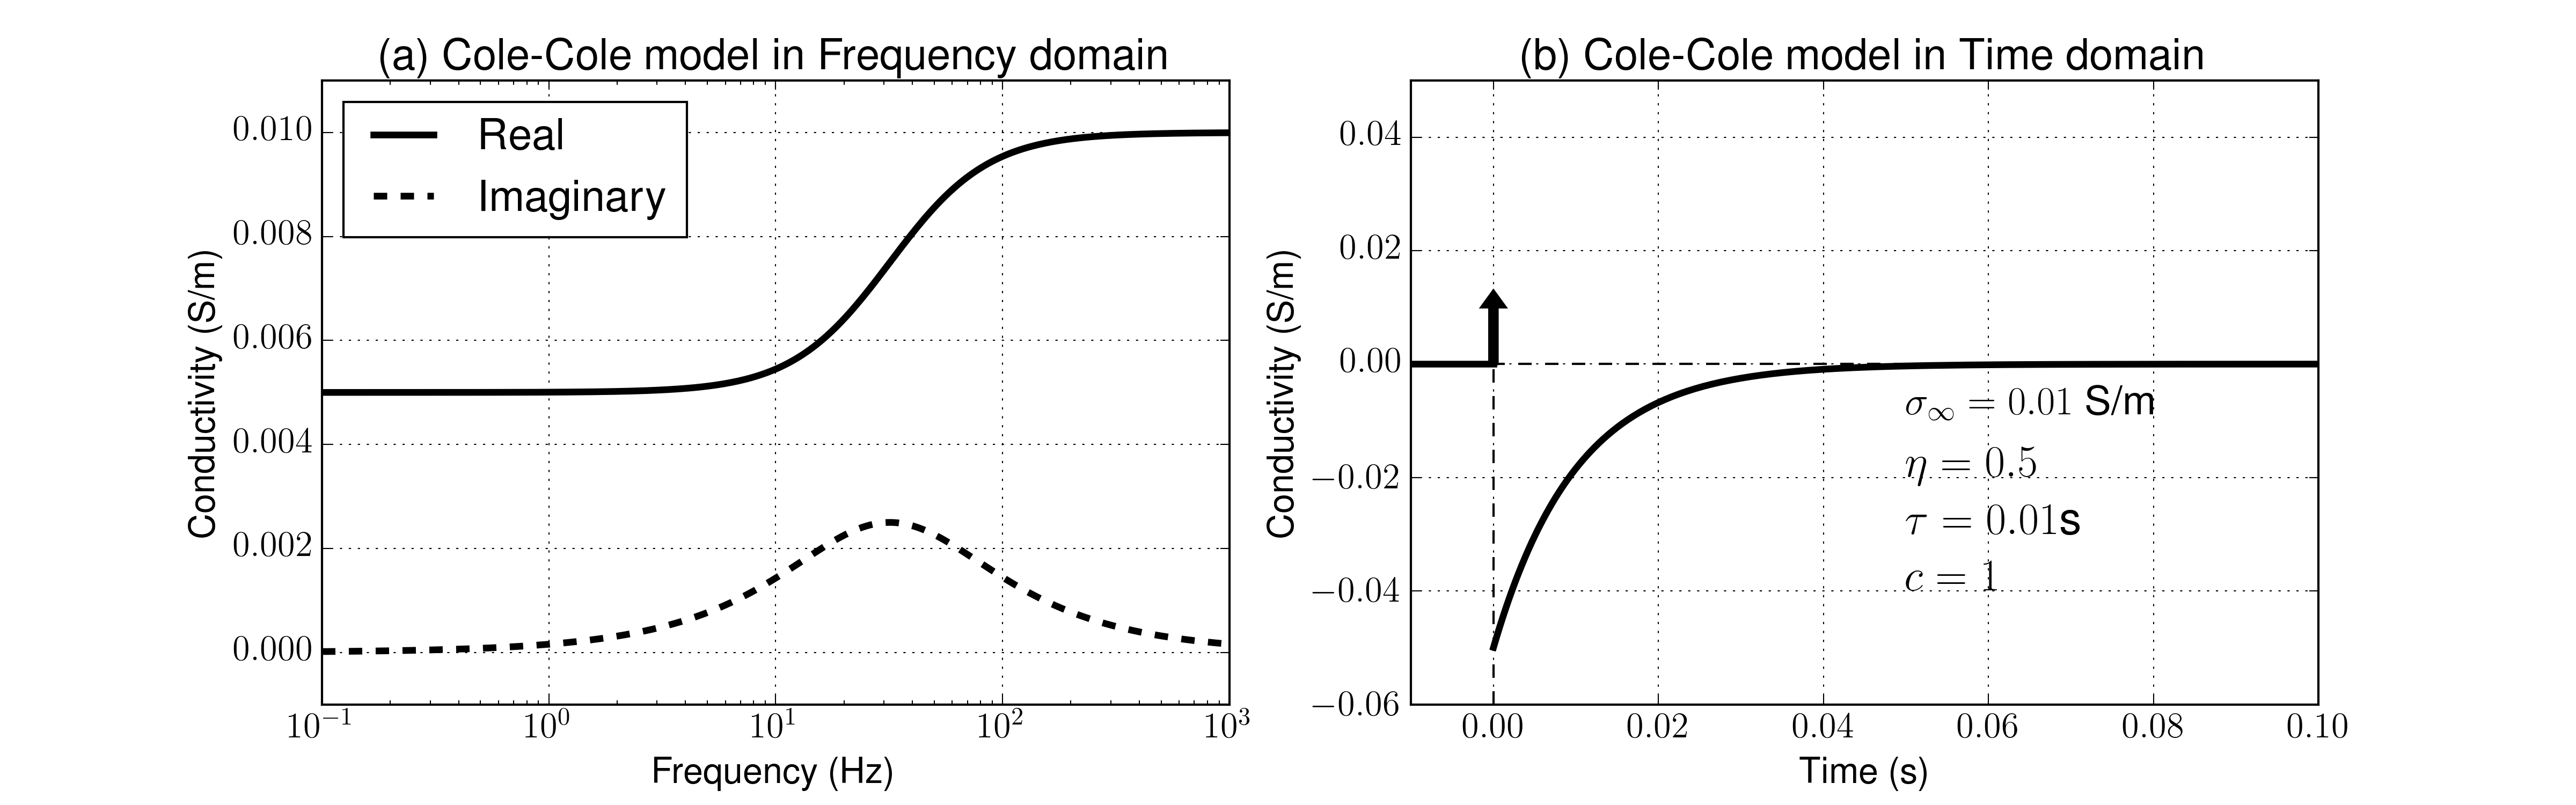
\includegraphics[width=1.0\textwidth]{figures/FDandTDCole.png}
  \caption{Cole-Cole model in frequency domain (a) and time (b) domain. }
  \label{Fig:FDandTDCole}
\end{figure}

%% =============================================================================
%% Section. Decomposition of EM responses
%% =============================================================================

\section{Decomposition of EM responses}
The basic ideas and notation presented thus far form the foundation of more general cases for grounded and airborne IP measurements. 
The difference arises because diffusion of the fields into the subsurface need to be taken into account and also electric fields due to the polarization can become important. 
Consider Maxwell's equations in time domain:
\begin{equation}
  \curl{\e} = -\frac{\partial \b}{\partial t}
  \label{eq: total_farad}
\end{equation}
\begin{equation}
  \curl{\frac{1}{\mu}\b} - \j= \j_{s},
  \label{eq: total_coulomb}
\end{equation}
where $\e$ is the electric field ($V/m$), $\b$ is the magnetic flux density ($Wb/m^2$) and $\mu$ is the magnetic permeability ($H/m$). Here $\j$ is the conduction current. In the frequency domain the current density $\J$ is related to conductivity via $\J(\omega) = \sigma(\omega)\E(\omega)$ where $\E$ is the electric field. Substituting equation (\ref{eq: sigma_freq}) yields:
\begin{equation}
  \J(\omega) = \sigma(\omega)\E(\omega).
\end{equation}
Converting this relationship to time domain using inverse Fourier transform yields:
\begin{equation}
  \j(t) = \sigma(t)\otimes \e(t),
  \label{eq: ohmslaw1}
\end{equation}
where $\otimes$ indicates time convolution. 
For causal signals, which is defined when $t \ge 0$, convolution between $a(t)$ and $b(t)$ can be written as
\begin{equation}
  a(t) \otimes b(t) = \int_0^t a(u) b(t-u) du.
  \label{eq: convolution}
\end{equation}
That is the current density depends upon the previous history of the electric field.
As in \cite{Smith1988a}, we let total fields as $\e = \e^{F} + \e^{IP}$, $\b = \b^{F} + \b^{IP}$ and $\j = \j^{F} + \j^{IP}$, where superscript $F$ indicates fundamental and $IP$ is induced polarization.
Substituting into equations (\ref{eq: total_farad}) and (\ref{eq: total_coulomb}) yields the following sequences:
\begin{equation}
  \curl({\e^{F}+\e^{IP}}) = -\frac{\partial}{\partial t} (\b^{F}+\b^{IP}),
\end{equation}
\begin{equation}
  \curl\frac{1}{\mu}(\b^{F}+\b^{IP}) - (\j^{F}+\j^{IP})= \j_{s}.
\end{equation}
By canceling out vectors associated with $EM$ terms, we have
\begin{equation}
  \curl \e^{IP} = -\frac{\partial \b^{IP}}{\partial t},
  \label{eq: eq_secondary_farad}
\end{equation}
\begin{equation}
  \curl{\frac{1}{\mu}\b^{IP}} = \j^{IP}.
  \label{eq: eq_secondary_coulomb}
\end{equation}
In addition, associated $EM$ equations can be written as
\begin{equation}
  \curl \e^{F} = -\frac{\partial \b^{F}}{\partial t},
  \label{eq: eq_primary_farad}
\end{equation}
\begin{equation}
  \curl{\frac{1}{\mu}\b^{F}} -\j^{F} = \j_s.
  \label{eq: eq_primary_coulomb}
\end{equation}
Here
\begin{equation}
  \j^{F} = \siginf\e^{F}.
  \label{eq: jF}
\end{equation}
Let $F[\cdot]$ denote operator associated with Maxwell’s equations and let $d$ denote the observed electromagnetic field thus, this includes both EM and IP effects. Keeping the same notation, we also write $d = d^{F} + \dip$. Therefore, we define IP datum as
\begin{equation}
  \dip = d - d^{F} = F[\siginf\delta(t)+\dsig(t)]-F[\siginf\delta(t)].
    \label{eq: IPdatum_syn}
\end{equation}
This subtraction process acts as an EM decoupling process, which reduces the EM effects in the measured responses. 
This formed the basis of work by \cite{routh2001}. 
Thus, assuming that we have a reasonable estimation for the distribution of $\siginf$ in 3D space, we can identify  IP datum, which are embedded in the observed responses. 

%% =============================================================================
%% Section. Linearization of EM responses
%% =============================================================================

\section{Linearization of EM responses}
A major difference of the inductive source from the galvanic source is the absence of the steady-state electric field. 
This generates a principal difference on the IP response for both inductive and galvanic sources. 
To carefully examine this, we define the IP current ($\j^{IP}$) as
\begin{equation}
  \j^{IP} = \siginf \e^{IP} + \j^{pol},
  \label{eq:IP_current}
\end{equation}
where the polarization current ($\j^{pol}$) is
\begin{equation}
  \j^{pol}(t) = \dsig(t) \otimes \e(t).
  \label{eq:polarization_current}
\end{equation}
The polarization current is the convolution between $\dsig (t)$ and the total electric field. 
Thus, if the electric field has different characteristic for the inductive and galvanic sources, this will be incorporated in the polarization current.
We consider two cases: a) galvanic source without EM induction and b) inductive source with EM induction. The first case corresponds to Electrical IP (EIP; Seigel), and the second one is ISIP.
Figure \ref{F:DCEM_F_current} shows the magnitude of the fundamental electric field ($\e^{F}$) in the earth for those two cases. 
For the galvanic source, the electric field is instantaneous due to the steady-state electric field (Figure \ref{F:DCEM_F_current} (a)). 
However, for the inductive source, the electric field on off-time is not zero, but increases to the peak then decays as shown in Figure \ref{F:DCEM_F_current} (b). 
The polarization current for two different sources will be significantly affected by these different electric fields. 
To capture this difference in the linearized kernel for the IP response, we define pseudo-chargeability ($\peta(t)$) as 
\begin{equation}
  \peta(t) = \frac{\j^{pol}(t)}{\j^{\ ref}},
  \label{eq:pseudochargeability_0}
\end{equation}
where the reference current ($\j^{ref}$) is defined as 
\begin{equation}
  \j^{\ ref} = \siginf \eref.
  \label{eq:reference_current}
\end{equation}
Here $\eref$ is the reference electric field. 
Both $\j^{\ ref}$ and $\eref$ are static field that is independent on time. 
The pseudo-chargeability is the fraction of the polarization current and the reference current. From the definition of the polarization current, we can simply expect magnitude of the IP response is proportional to that of the pseudo-chargeability, and it varies in time. 
The pseudo-chargeability is an important property because we are going to linearize IP response as a function of the pseudo chargeability. 
To evaluate the pseudo-chargeability, we have to identify the reference current or electric fields. 
For the EIP case, the choice of the reference current is obvious because the electric field is independent on time without IP effect as shown in Figure \ref{F:DCEM_F_current}a). 
We choose the fundamental electric field of on-time. 
For the inductive source, the electric field does not reach to the steady-state, but increases to the peak then decreases. Thus an intuitive choice of the reference electric field can be the maximum of the $\e^{F}$. This maximum electric field ($\eFmax$) and the maximum time ($t^{max}$) when it occurs are going to be different in each pixel of the earth. 
Accordingly, both $\eFmax$ and $t^{max}$ have 3D distribution. 
For both EIP and ISIP cases, we mathematically our choice of the reference field as
\begin{equation}
  \eref = \eFmax = \e^{F}(t) \otimes \delta(t-t^{max}). 
\end{equation}
The reference current can be simply defined as $\j^{\ ref}  = \siginf \eref$. 
Since the fundamental electric field for EIP case is independent on time above equation still holds. 

\begin{figure}
  \centering  
  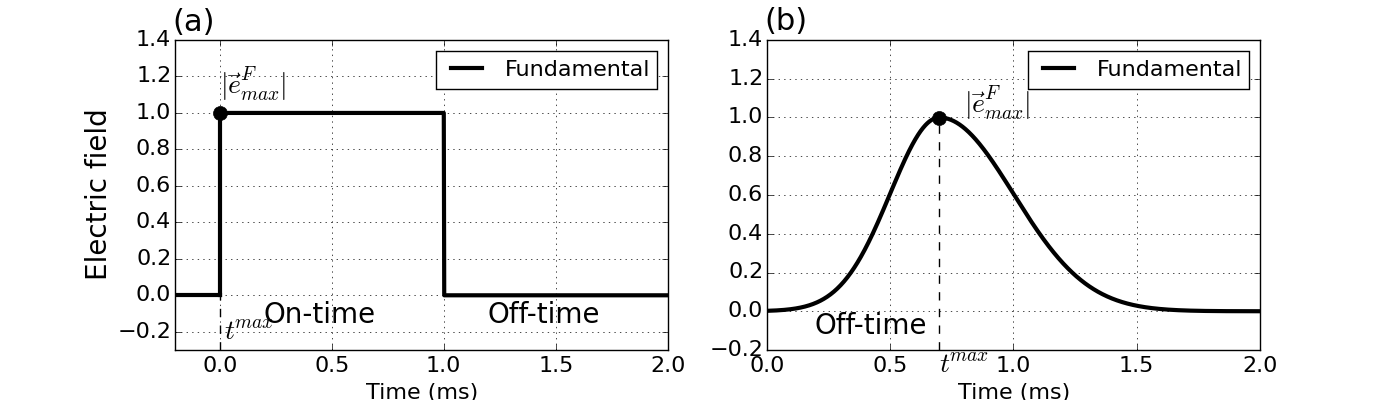
\includegraphics[width=1.0\textwidth]{figures/DCEM_F_current.png}
  \caption{Conceptual diagram for the amplitude of the fundamental electric fields. (a) EIP and (b) ISIP cases.}
  \label{F:DCEM_F_current}
\end{figure}
  

%% =============================================================================
%% Sub-Section. Linearization 

\subsection{Linearization}
Our goal of the linearization is to express $\dip$ as a function of the pseudo-chargeability $(\peta(t))$ in time. 
Therefore, we can have a form of linear equation like $\dip(t) = -J[\peta(t)]$, where $J[\cdot]$ is a linear operator, which is independent on time. 
A strategy of our linearization as follows: 1) Linearize the IP current as a function of the pseudo-chargeability. 2) Use Biot-Savart law to evaluate IP magnetic flux density or its time derivative. 

Although this study focuses on IP for ATEM survey, for the linearization of IP responses, we consider a general EM system, which can be either galvanic and inductive sources. 
Let the total electric field, $\e(t)$ can be approximated as
\begin{equation}
  \e(t) \approx \eref w^e(t),
  \label{eq: e_with_eref}
\end{equation}
where $w^e(t)$ is defined as:
\begin{equation}
  w^e(t) = \left\{ 
  \begin{array}{l l}
    w^{ref}(t) & w^{ref}(t) \ge 0 \\
    0 & \text{if } w^{ref}(t) < 0, 
  \end{array}\right.
  \label{eq: we}
\end{equation}
with
\begin{equation}
  w^{ref}(t) = \frac{\e(t)\cdot\eref}{\eref\cdot\eref}.
  % \label{eq: we}
\end{equation}
Here $w^{ref}(t)$ is a dimensionless function that prescribes the time history of the electric field at each location and the reference electric field ($\eref$) is an appropriate scaling for the electric field, which is independent on time. 
This indicates that the direction of the electric field does not change in time. 
In addition, by the definition of $w^e(t)$, we projects negatives values of  $w^{ref}(t)$ to zero.
Note that this assumption is only applied to the second term on right-hand side of equation (\ref{eq:IP_current}). 
Substituting this into equation (\ref{eq:IP_current}) yields
\begin{eqnarray*}
  \j^{IP}(t) \approx \siginf\e^{IP}(t) + \frac{\dsig(t)\otimes w^e(t)}{\siginf}\j^{\ ref},
\end{eqnarray*}
where the reference current density is defined as
\begin{equation}
  \j^{ref} = \siginf\eref.
\end{equation}
Letting pseudo-chargeability as
\begin{equation}
    \peta(t) = -\frac{\dsig(t)\otimes w^e(t)}{\siginf} \approx -\frac{\j^{pol}}{\j^{\ ref}},
    \label{eq: pseudochargeability}
\end{equation}
we obtain
\begin{eqnarray}
  \j^{IP}(t) = \siginf\e^{IP}(t) + \j^{pol}(t) \approx \siginf\e^{IP}(t) -\j^{\ ref}\peta(t).
  \label{eq: jip_EMIP}
\end{eqnarray}
A physical insight about the pseudo-chargeability is that a fraction of polarization current and reference current. Because the reference current is time-independent property, any time-dependency in the pseudo-chargeability is from the polarization current. Using Helmholtz decomposition, $\e$ can be decomposed as $\e=-\vec{a}-\grad\phi$, where $\vec{a}$ and $\phi$ is electric vector and scalar potentials, respectively and $\div\vec{a}=0$. Physically, those two terms indicate charge-build up and EM induction effects, which induce galvanic and vortex currents, respectively. So, $\e^{IP}$ can be decomposed as
\begin{equation}
  \e^{IP}=-\vec{a}^{IP}-\grad\phi^{IP}.
\end{equation}
Now we make another assumption:
\begin{equation}
  \e^{IP} \approx  \e^{IP}_{approx} = -\grad\phi^{IP},
  \label{eq: eip_approx}
\end{equation}
which means $\e^{IP}$ term in equation (\ref{eq: jip_EMIP}) is dominated by galvanic effect ($\frac{\partial\b^{IP}}{\partial t}\approx 0$). First taking $\div$ to equation (\ref{eq: jip_EMIP}) then by substituting  $\e^{IP}$ with equation (\ref{eq: eip_approx}) with some linear algebra, we obtain
\begin{equation}
  \phi^{IP}(t) \approx -[\div \siginf\grad]^{-1}\div\j^{\ ref}\peta(t).
  \label{eq: phiIPapprox_general}
\end{equation}
By taking $\grad$ to this equation we have
\begin{equation}
    \e^{IP}_{approx} = \grad[\div \siginf\grad]^{-1}\div\j^{\ ref}\peta(t).
    \label{eq: eip_approx_full}
\end{equation}
Thus, the electric field due to the IP effect can be expressed as a function of $\peta(t)$ in time.

The observed data can be $\b$ or $\frac{\partial \b}{\partial t}$ in some cases thus, we need to compute $\b^{IP}$ or $\frac{\partial \b^{IP}}{\partial t}$.
 For this, we first compute $\j^{IP}$ then use Biot-Savart law to compute $\b^{IP}$ or $\frac{\partial \b^{IP}}{\partial t}$. 
Substituting equation (\ref{eq: phiIPapprox_general}) into equation (\ref{eq: jip_EMIP}), approximated IP current density, $\j^{IP}_{approx}$ can be expressed as
\begin{equation}
  \j^{IP}(t) \approx \j^{IP}_{approx} = -\bar{S}\siginf\eref\peta(t),
  \label{eq: jip_approx}
\end{equation}
where
\begin{equation}
  \bar{S} = -\siginf\grad[\div \siginf\grad]^{-1}\div+\bar{I}
\end{equation}
and $\bar{I}$ is an identity tensor. Then by using Biot-Savart law we have:
\begin{equation}
  \b^{IP}_{approx}(\vec{r}; t) = -\frac{\mu_0}{4\pi}\int_{\Omega}  \frac{\bar{S}\eref(\vec{r}_s)\times\hat{r}}{|\vec{r}-\vec{r}_s|^2}\peta(t)d\vec{r}_s.
  \label{eq: BiotbIP_approx}
\end{equation}
By taking time derivative to the above equation we have
\begin{equation}
  \frac{\partial\b^{IP}_{approx}}{\partial t}(\vec{r}) = -\frac{\mu_0}{4\pi} \int_{\Omega}  \frac{\bar{S}\eref(\vec{r}_s)\times\hat{r}}{|\vec{r}-\vec{r}_s|^2}\frac{\partial}{\partial t}\peta(t)d\vec{r}_s.
  \label{eq: BiotbIPdt_approx}
\end{equation}
Various types of the IP fields shown in equations (\ref{eq: eip_approx_full}), (\ref{eq: BiotbIP_approx}) and (\ref{eq: BiotbIPdt_approx}) are function of $\peta(t)$.
The time dependency only rises from $\peta(t)$. 
To summarize, with the assumption that $\e^{IP}$ is mostly galvanic, we show that IP fields can have linear relationship with $\peta(t)$. Therefore, $\dip$ responses, which can be any type of electromagnetic fields, can be represented as $\dip(t) = -J[\peta(t)]$. In discretized space this can be expressed as
\begin{equation}
  \mathbf{d}^{IP}_i = -\mathbf{J}\peta_i,
  \label{eq: dIP_lineareq}
\end{equation}
where $\mathbf{J}$ is corresponding sensitivity matrix and the subscript $i$ indicates $i^{th}$ time channel. 
Boldface of upper and lower cases indicate a matrix and column vector in discretized space. Since $\dip$ can be any types of electromagnetic fields, our approach to linearize time domain IP responses is applicable for any types of TEM surveys, whereas some details for practical application might be somewhat different. 
However, the fundamental concept will be same. 
On the other hand, we must carefully investigate the assumptions that we have made to formulate this linear relationship, and characteristics of the pseudo-chargeability.

%% =============================================================================
%% Section. IP inversion methodology
%% =============================================================================

\section{IP inversion methodology}

%%% ===========================================================================
%%% SUBSECTION
\subsection{IP inversion procedure}
The IP inversion of ATEM data can have multiple steps including some processings and the application of the 3D inversion. We suggest a procedure of the 3D IP inversion for ATEM data as following.
To obtain the fundamental EM response, $d^F$, (1) invert ATEM data and recover a 3D conductivity model ($\sigma_{est}$). 
This may involve omitting data that are obviously contaminated with IP signals, such as the existence of negative transients in coincident loop surveys. 
(2) Forward modelling then yields an approximate value of $d^F$ and subtract it from the observations, $d$. 
However, we cannot obtain the correct $d^F$, since the estimated conductivity is not exact. 
(3) Therefore the computed $\dip$ data may have some errors containing both a residual field due to the incorrect conductivity and some noises. This residual field potentially need to be removed with some processings. 
The final data are linearly related to a pseudo-chargeability through a sensitivity function shown in equation (\ref{eq: dIP_lineareq}). 
(4) The $\dip$ at various time channels can be inverted individually. The pseudo-chargeability models may be useful in themselves or they can be further processed to estimate Cole-Cole, or equivalent IP parameters.

%%% ===========================================================================
%%% SUBSECTION
\subsection{Equivalent pseudo-chargeability}
We derived a linearized kernel function of $\dip$ response as a function of the pseudo-chargeability ($\peta(t)$) for general TEM surveys. 
An important point of this derivation is that the pseudo-chargeability is defined for each sounding that is, they are different for each sounding. 
This indicates that IP response should be defined as 
\begin{equation}
  \dip_k(t) = J_k[\peta_k (t)], \ \ k=1, \ldots, nTx,
\end{equation}
the subscript $k$ indicates $k$-th sounding and $nTx$ is the number of soundings. This  induces a significant problem for ATEM case because this survey contains numerous soundings.
Setting up an inverse problem for 3D pseudo-chargeability of each sounding will cause extremely non-unique inverse problem. 
To effectively deal with this issue, we suggest an equivalent pseudo-chargeability ($\peta_{eqv}$), which represents pseudo-chargeability from every sounding with reasonable explanation of the IP responses. 

From the definition shown in equation (\ref{eq: pseudochargeability}), we recognize that the pseudo-chargeability is fraction of the polarization and the reference current. 
Using the normalization of the polarization current with the reference current, which will be different for each sounding, we make our best to express the pseudo-chargeability as an independent property for each sounding. 
This will mainly depend on $w^e(t)$, because the pseudo-chargeability is the convolution between $\peta^{I}(t)$ and $w^e(t)$:
\begin{equation}
  \peta_k(t) = \peta^{I}(t) \otimes w^e_k(t),
  \label{eq: pseudochargeability_petaI}
\end{equation}
Therefore, if $w^e_k$ is identical for every sounding, then we can let $\peta_{eqv} = \peta_k$, $k=1, \ldots, nTx$. 
Based on this, we obtain a linear equation for IP responses as
\begin{equation}
  \dip_i =J[\peta_{eqv \ i}],
  \label{eq: pseudochargeability_equivalent}
\end{equation}
where the sensitivity function, $J[\cdot]$ takes $\peta_{eqv \ i}$, and outputs $\dip_i$ responses for all soundings at the $i$-th time. 
Reliability of the equivalent pseudo-chargeability for ATEM survey should be carefully investigated. 

%%% ===========================================================================
%%% SUBSECTION
\subsection{3D IP inversion with linearized kernel}
To set up an linear inverse problem we rewrite equation (\ref{eq: dIP_lineareq}) as
\begin{eqnarray}
  \mathbf{d}^{pred} = \mathbf{A}\mathbf{m},
  \label{eq9}
\end{eqnarray}
where $\mathbf{A}$ is sensitivity matrix of linear problem, which corresponds to $\mathbf{J}$ shown in equation (\ref{eq: dIP_lineareq}) 
Here, $\mathbf{d}^{pred}$ is IP responses at $i^{th}$ time channel ($\mathbf{d}^{IP}_i$), $\mathbf{m}$ is distributed model parameters, which can be either $\peta_{i}$ or $\frac{\partial}{\partial t}\peta_{i}$. 
This presents that we invert each time channel of $d^{IP}$, separately. 
Our inversion methodology is based upon that described in \cite{doug1994}. The solution to the inverse problem is the model $\mathbf{m}$ that solves the optimization problem
\begin{eqnarray}
  minimize \ \phi =  \phi_d(\mathbf{m}) + \phi_m(\mathbf{m})\nonumber \\
  s.t. \ 0 \le \mathbf{m},
  \label{eq10}
\end{eqnarray}
where $\phi_d$ is a measure of data misfit, $\phi_m$ is a user defined model objective function and $\beta$ is regularization or trade-off parameter. 
We use the sum of the squares to measure data misfit
\begin{eqnarray}
  \phi_d = \| \mathbf{W_d}(\mathbf{A}\mathbf{m}-d^{obs}|)\|^2_2 =
  \sum^N_{j=1}(\frac{\mathbf{d}^{pred}_j-\mathbf{d}^{obs}_j}{\epsilon_j}),
  \label{eq11}
\end{eqnarray}
where $N$ is the number of the observed data and $\mathbf{W_d}$ is a diagonal data weighting matrix which contains the reciprocal of the esitmated uncertainty of each datum (
$\epsilon_j$) on the main diagonal,  $\mathbf{d}^{obs}$ is a vector containing the observed data, $\mathbf{d}^{pred}$ is a vector containing calculated data from a linear equation given in equation (\ref{eq9}).
The model objective function, $\phi_m$ is a measure of amount structure in the model and upon minimization this will generate a smooth model which is close to a reference model, $m_{ref}$. 
We define $\phi_m$ as
\begin{eqnarray}
  \phi_m = \alpha_s\| \mathbf{W}_s\mathbf{W}(\mathbf{m}-\mathbf{m}_{ref})\|^2_2+
       \alpha_x\| \mathbf{W}_x\mathbf{W}(\mathbf{m}-\mathbf{m}_{ref})\|^2_2+ \nonumber \\
       \alpha_y\| \mathbf{W}_y\mathbf{W}(\mathbf{m}-\mathbf{m}_{ref})\|^2_2+
       \alpha_z\| \mathbf{W}_z\mathbf{W}(\mathbf{m}-\mathbf{m}_{ref})\|^2_2,
  \label{eq12}
\end{eqnarray}
where $\mathbf{W}_s$ is a diagonal matrix, and $\mathbf{W}_x$, $\mathbf{W}_y$ and $\mathbf{W}_z$ are discrete approximations of the first derivative operator in $x$, $y$ and $z$ directions, respectively.  
The $\alpha$'s are weighting parameters that balance the relative importance of producing small or smooth models. We are inverting each time channel of $\dip$ datum, separately. Thus, we may not have intrinsic depth resolution in the inversion. To compensate this, similar to magnetic inversion (\cite{LiMag3D}), we apply depth weighting through model weighting matrix ($\mathbf{W}$):
\begin{equation}
    \mathbf{W} = \mathbf{diag}(\mathbf{z-z_0})^{1.5},
    \label{eq: weight_mat}
\end{equation}
where $\mathbf{z}$ and $\mathbf{z_0}$ are discretized depth locations and reference depth in 3D domain.

\subsection{Extracting intrinsic IP parameters}

Output of our IP inversion is 3D distribution of the pseudo-chargeability at multiple time channels. 
Thus the recovered pseudo-chargeability can be considered as 4D property. 
As its name suggests, pseudo-chargeability is not intrinsic IP parameters like chargeability, but convoluted property between $\peta^{I}(t)$ and $w^{e}(t)$ as shown in equation \ref{eq: pseudochargeability_petaI}. 
Assuming Debye model ($c$=1), we obtain
\begin{equation}
    \peta^{I}(t) = \frac{\eta}{(1-\eta)\tau}e^{-\frac{t}{(1-\eta)\tau}}u(t),
    \label{eq: intrinsic_peta_debye}
\end{equation}
where $u(t)$ is Heaviside step function. 
Since should have information about 3D conductivity after 3D IP inversion, we can compute  $w^e(t)$, which is time history of the electric field. 
Accordingly, we can unravel recovered pseudo-chargeability to recover intrinsic IP parameters such as chargeability($\eta$) and time constant ($\tau$). 
This will include solving an inverse problem for each cell. 

%% =============================================================================
%% Section. Numerical experiments
%% =============================================================================

\section{Numerical experiments}

\subsection{IP responses and currents}



\subsection{Validation of the linearization}



\subsection{3D IP inversion}



\subsubsection{Equivalent pseudo-chargeability}



\subsubsection{Depth weight and positivity constraint}



\subsubsection{Incorrect conductivity}



\subsubsection{Extracting intrinsic IP parameters}



\bibliographystyle{plain}
\bibliography{reference}

\end{document}



